\section{Results from test runs}
\label{sec:resul}
All the results shown below are derived by running FjordOs CL on the Vilje supercomputer at the Norwegian High Performance Computing facilities in Trondheim. We show results from a hindcast initialized from NorKyst800 on April 1st, 2014 and continued up to and including the month of December 2015. 
All inputs are as described in Section \ref{subsec:atmos}.
 
The results from the hindcast are further discussed and evaluated in some detail in an upcoming report \citep{hjelm:etal:2016}. Here we merely present snapshots of fields of currents, temperature, salinity and sea level so as to properly appreciate the level of details that the FjordOs CL model provides. In this we focus on six areas, namely the Inner Oslofjord, the Drammensfjord, the {\DR} area (henceforth {\DR}), the mid part of the Oslofjord (henceforth Slagen), the outer western part (henceforth Tristein) and the outer eastern part of the Oslofjord (henceforth Hvaler). 

\clearpage
%\subsubsection{Currents}
 %%%%%%%%%%%%%%%%%%% Figure  %%%%%%%%%%%%%%%
\begin{figure}[t]
  \begin{pspicture}(0,0)(15,12)
% Include graphs
	\rput[b](7.5,0){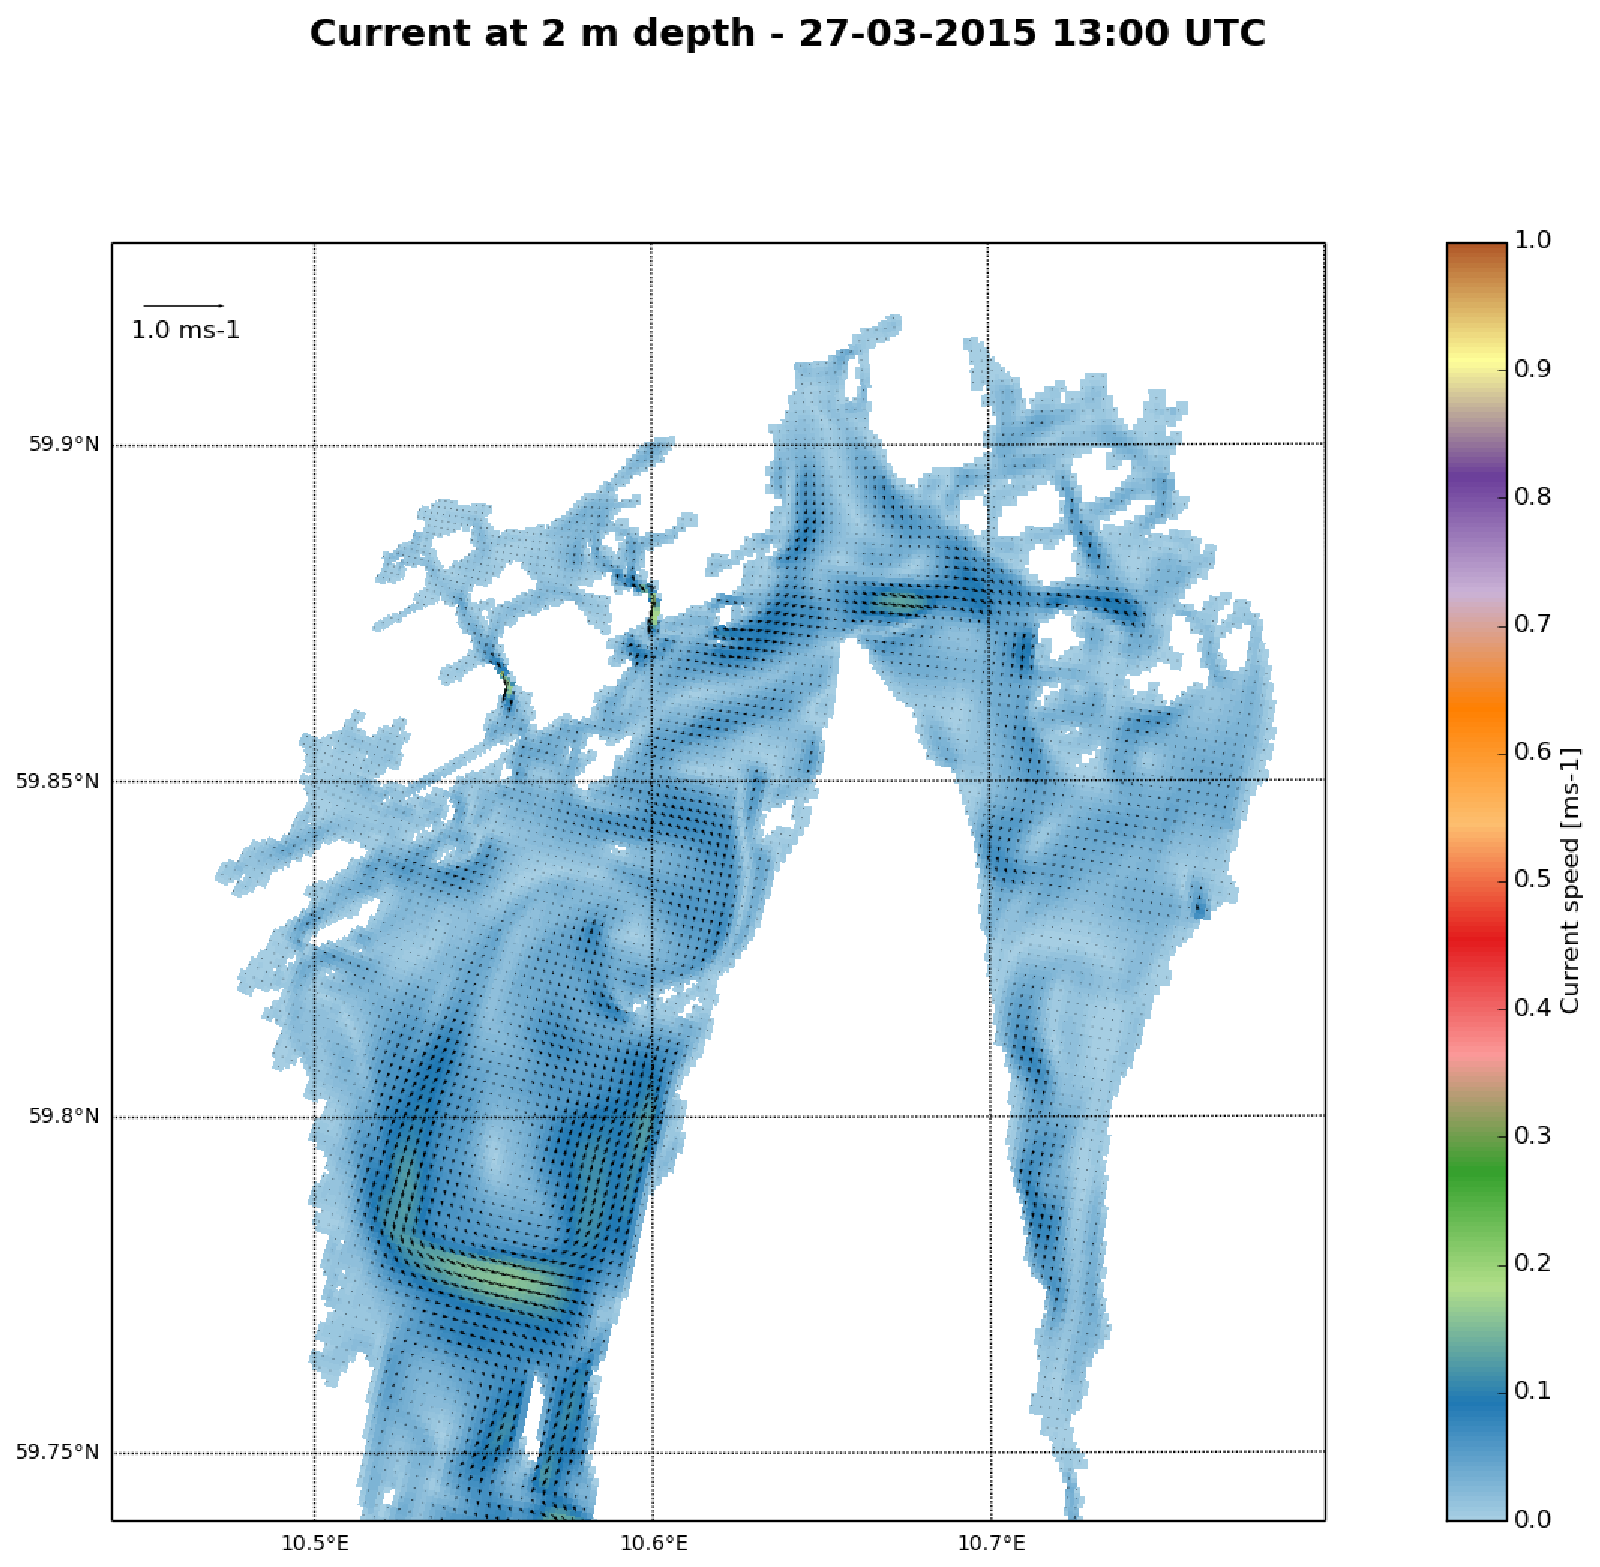
\includegraphics[height=12cm]{kap5/ferder1__0_current_crop}}
  \end{pspicture}
  \caption{\small  Currents .  }
  \label{fig:curr_oslo}
\end{figure}

  
 %%%%%%%%%%%%%%%%%%% Figure  %%%%%%%%%%%%%%%
\begin{figure}[t]
  \begin{pspicture}(0,0)(15,14)
% Include graphs
	\rput[b](7.5,-0.5){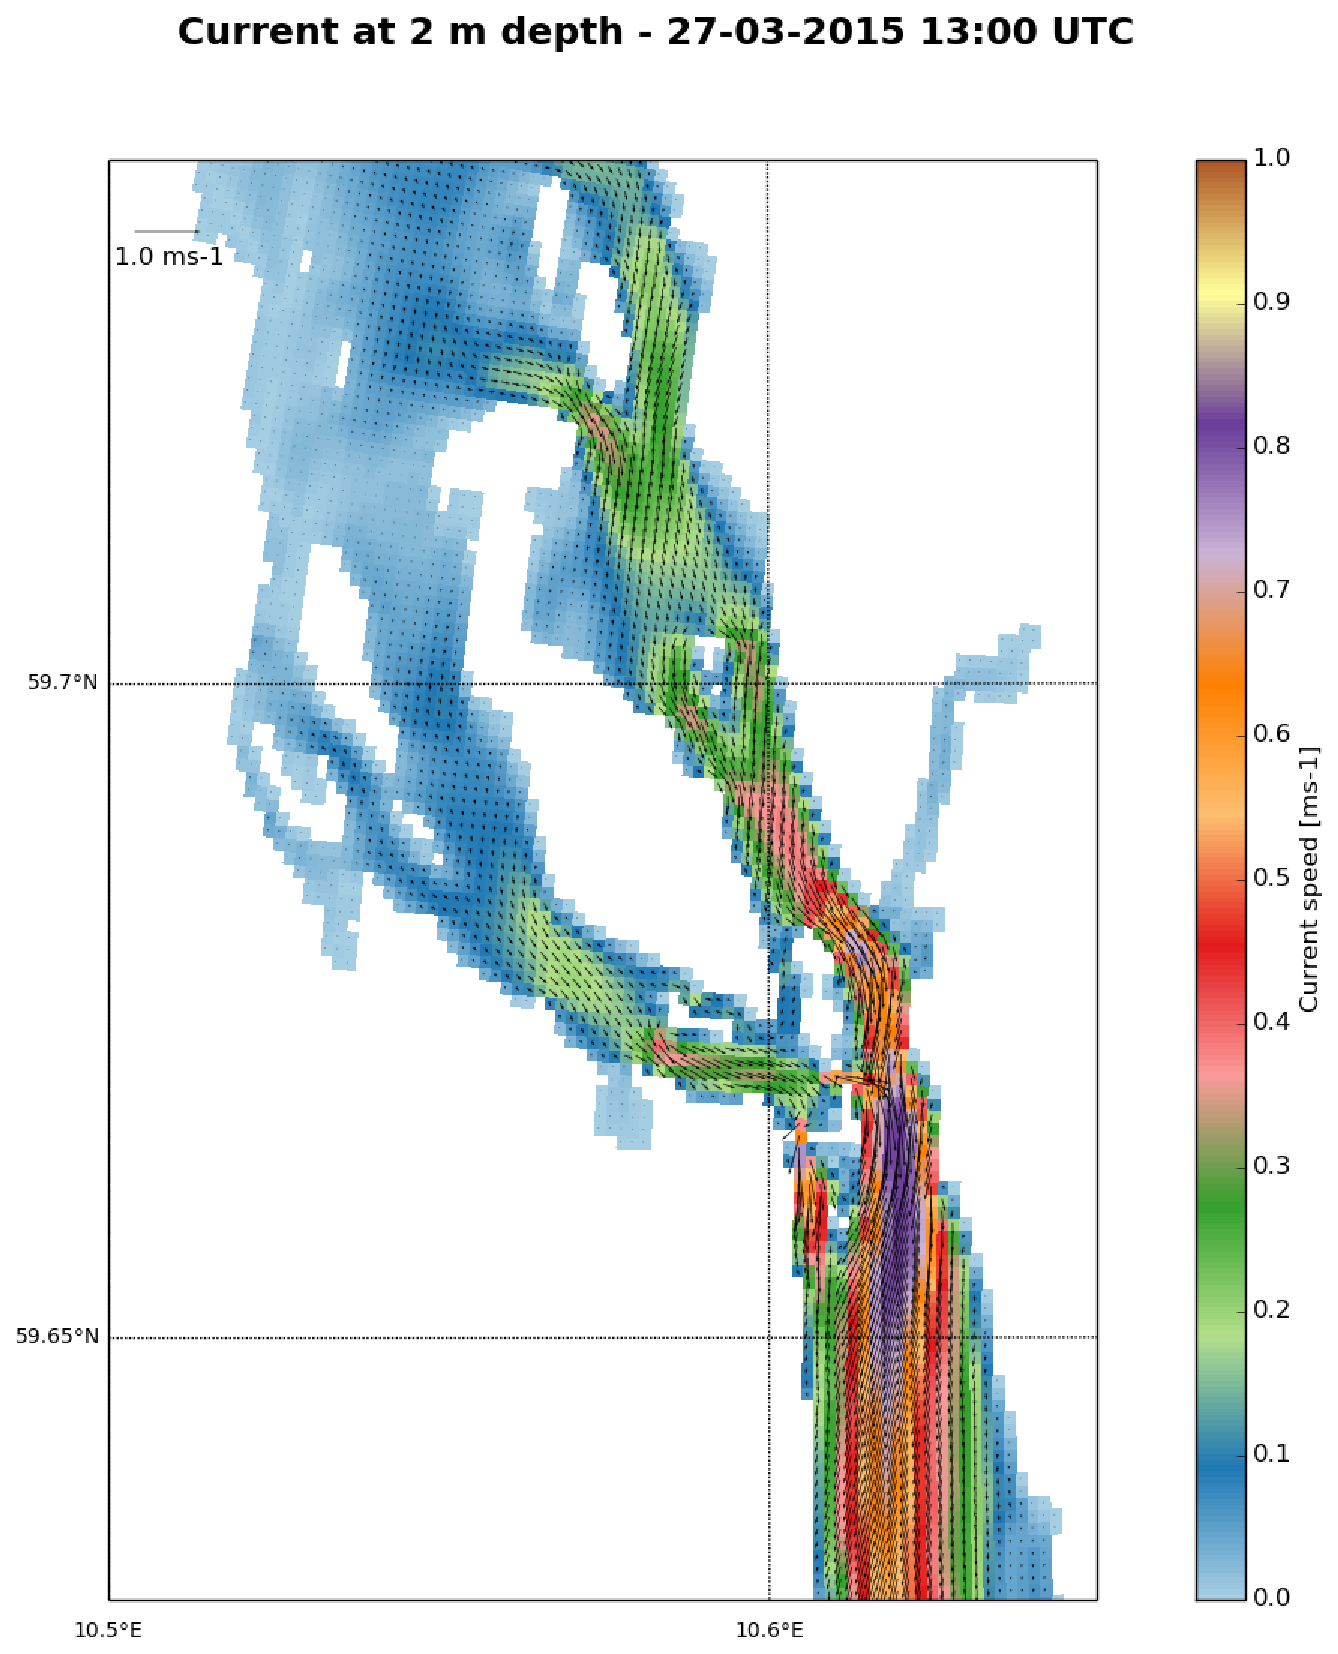
\includegraphics[height=14.5cm]{kap5/ferder2__0_current_crop}}
  \end{pspicture}
  \caption{\small As Figure \ref{fig:curr_oslo}, but for the Dr{\o}bak Sound and Vestfjorden area.}
  \label{fig:curr_drobak}
\end{figure}

  
 %%%%%%%%%%%%%%%%%%% Figure  %%%%%%%%%%%%%%%
\begin{figure}[t]
  \begin{pspicture}(0,0)(15,12)
% Include graphs
	\rput[b](7.5,0){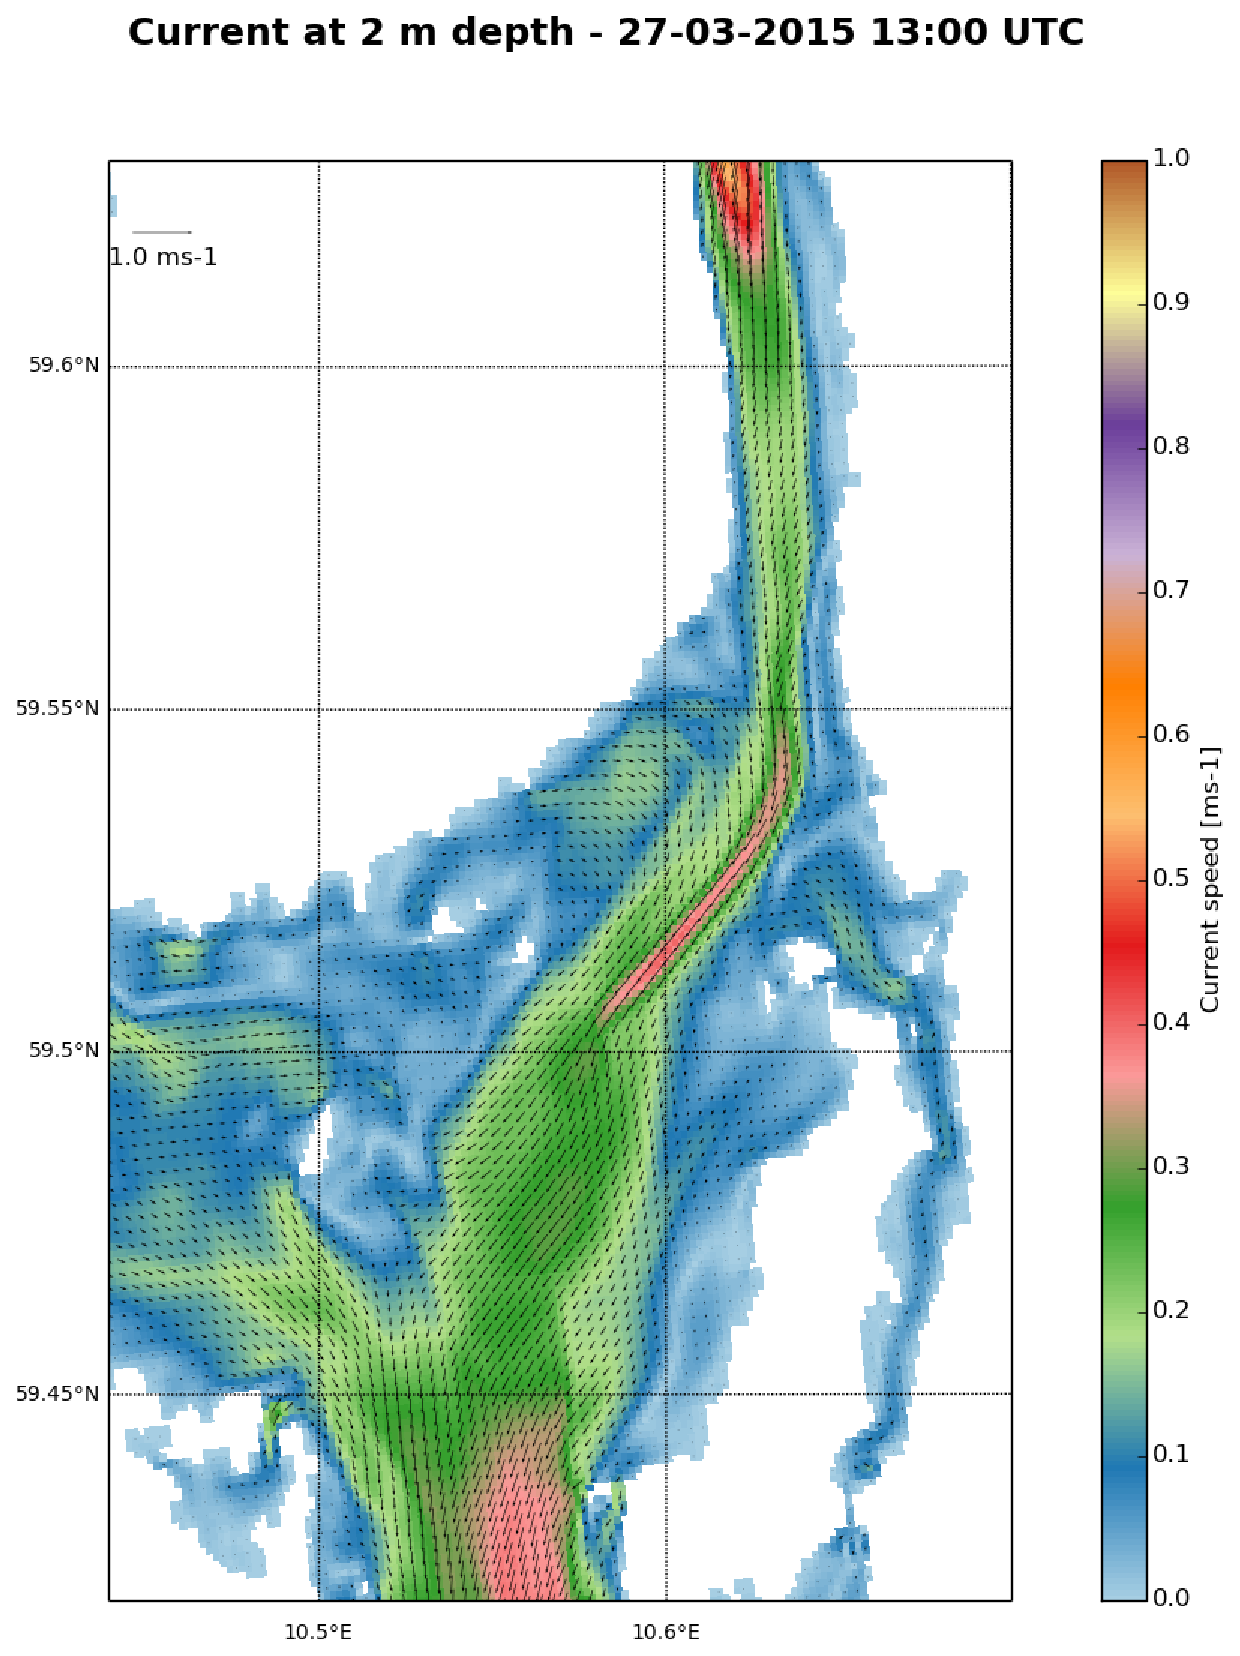
\includegraphics[height=12cm]{kap5/ferder3__0_current_crop}}
  \end{pspicture}
  \caption{\small  As for figure \ref{fig:curr_oslo}, but for the southern part of the Dr{\o}bakssund and Breidangen area.  }
  \label{fig:curr_breiangen}
\end{figure}

  
 %%%%%%%%%%%%%%%%%%% Figure  %%%%%%%%%%%%%%%
\begin{figure}[t]
  \begin{pspicture}(0,0)(15,16)
% Include graphs
	\rput[b](7.5,0){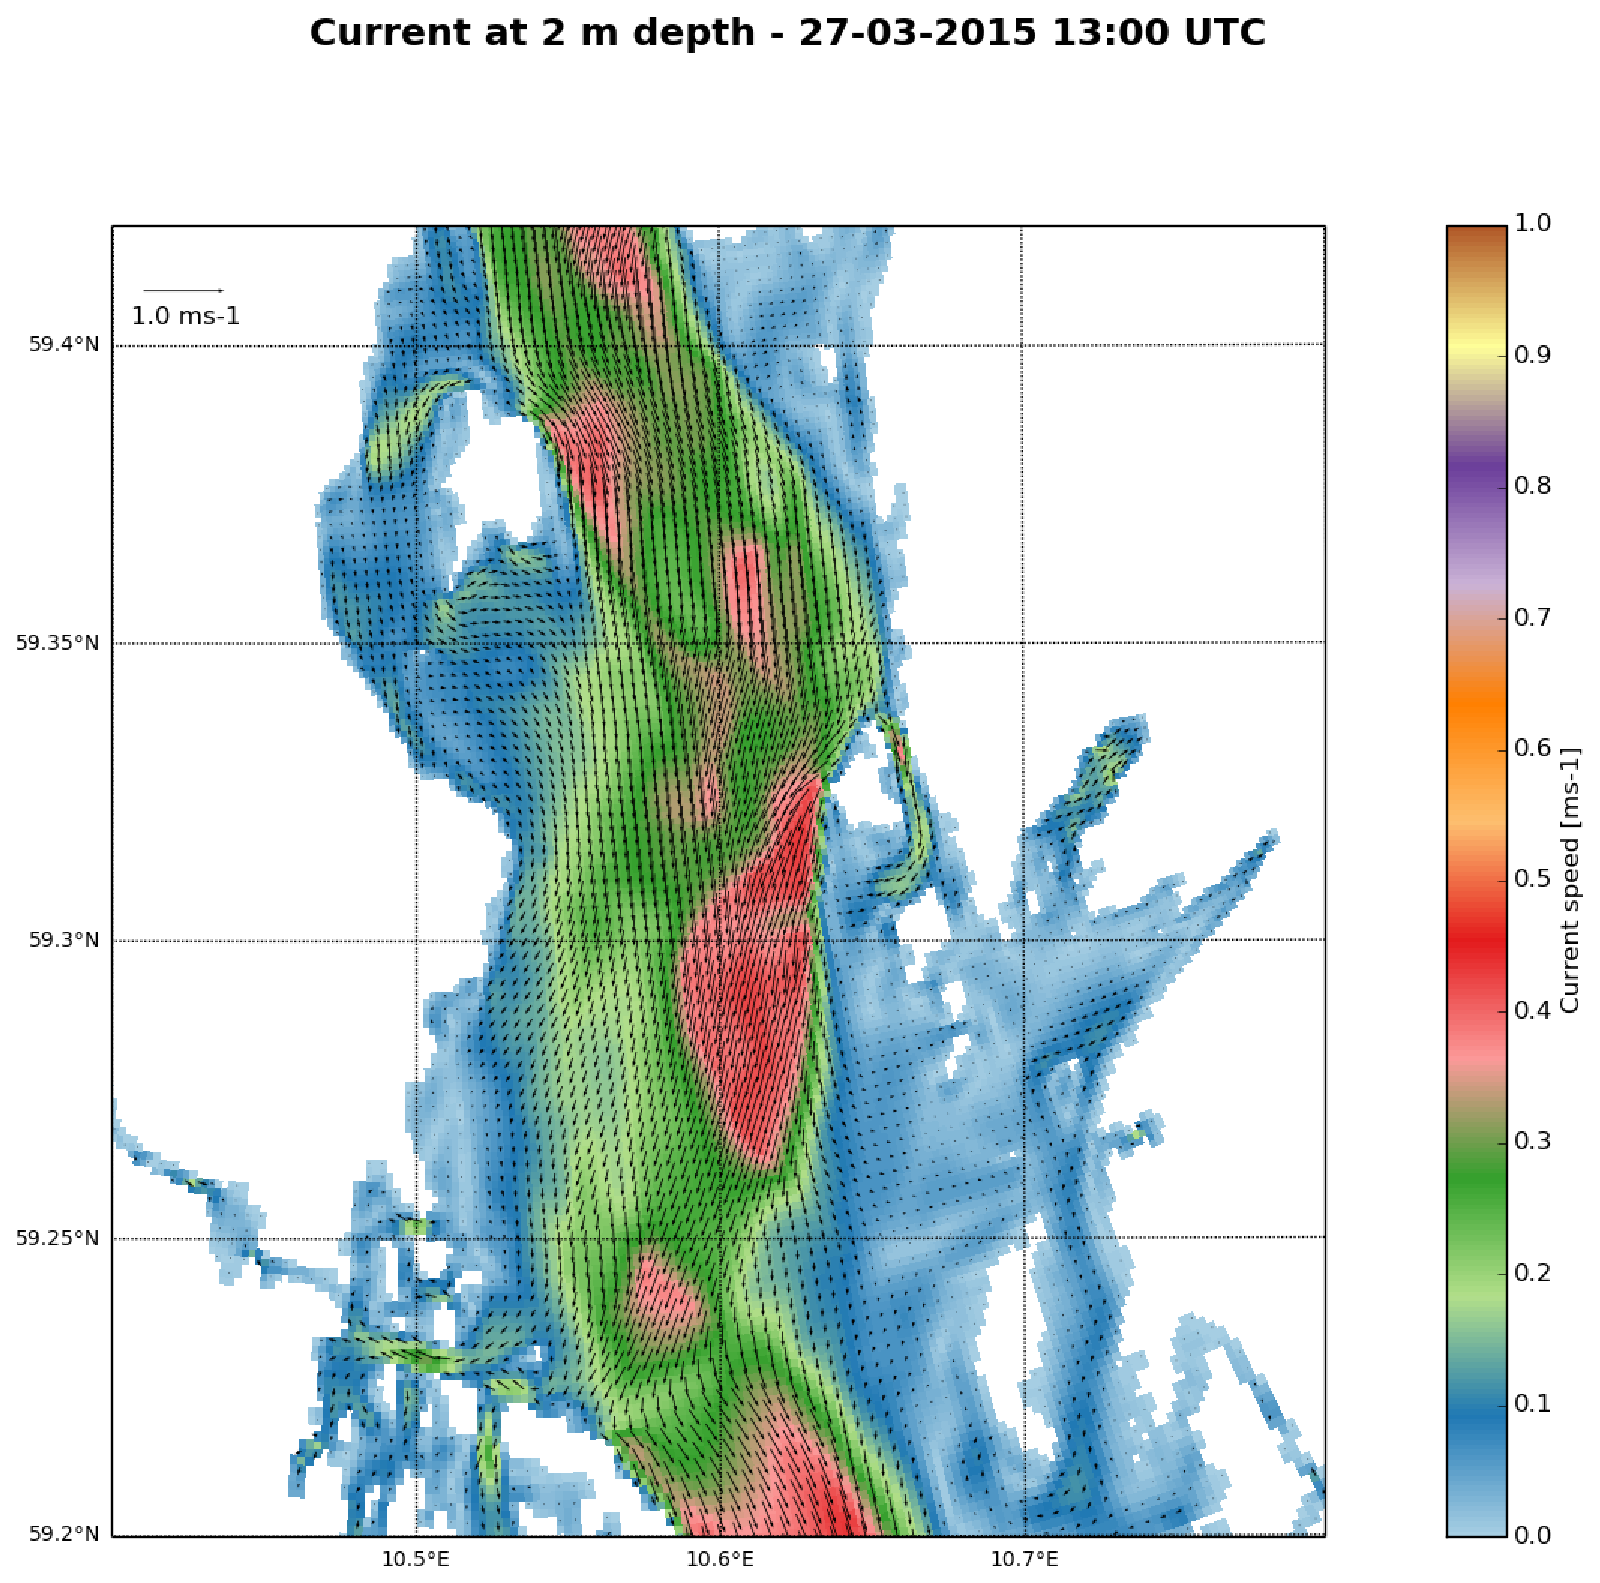
\includegraphics[height=16cm]{kap5/ferder4__0_current_crop}}
  \end{pspicture}
  \caption{\small  As Figure \ref{fig:curr_oslo}, but for the area between the Bast{\o}y, Rauer and Bol{\ae}rne islands.  }
  \label{fig:curr_mefjord}
\end{figure}

  
 %%%%%%%%%%%%%%%%%%% Figure  %%%%%%%%%%%%%%%
\begin{figure}[t]
  \begin{pspicture}(0,0)(15,12)
% Include graphs
	\rput[b](7.5,0){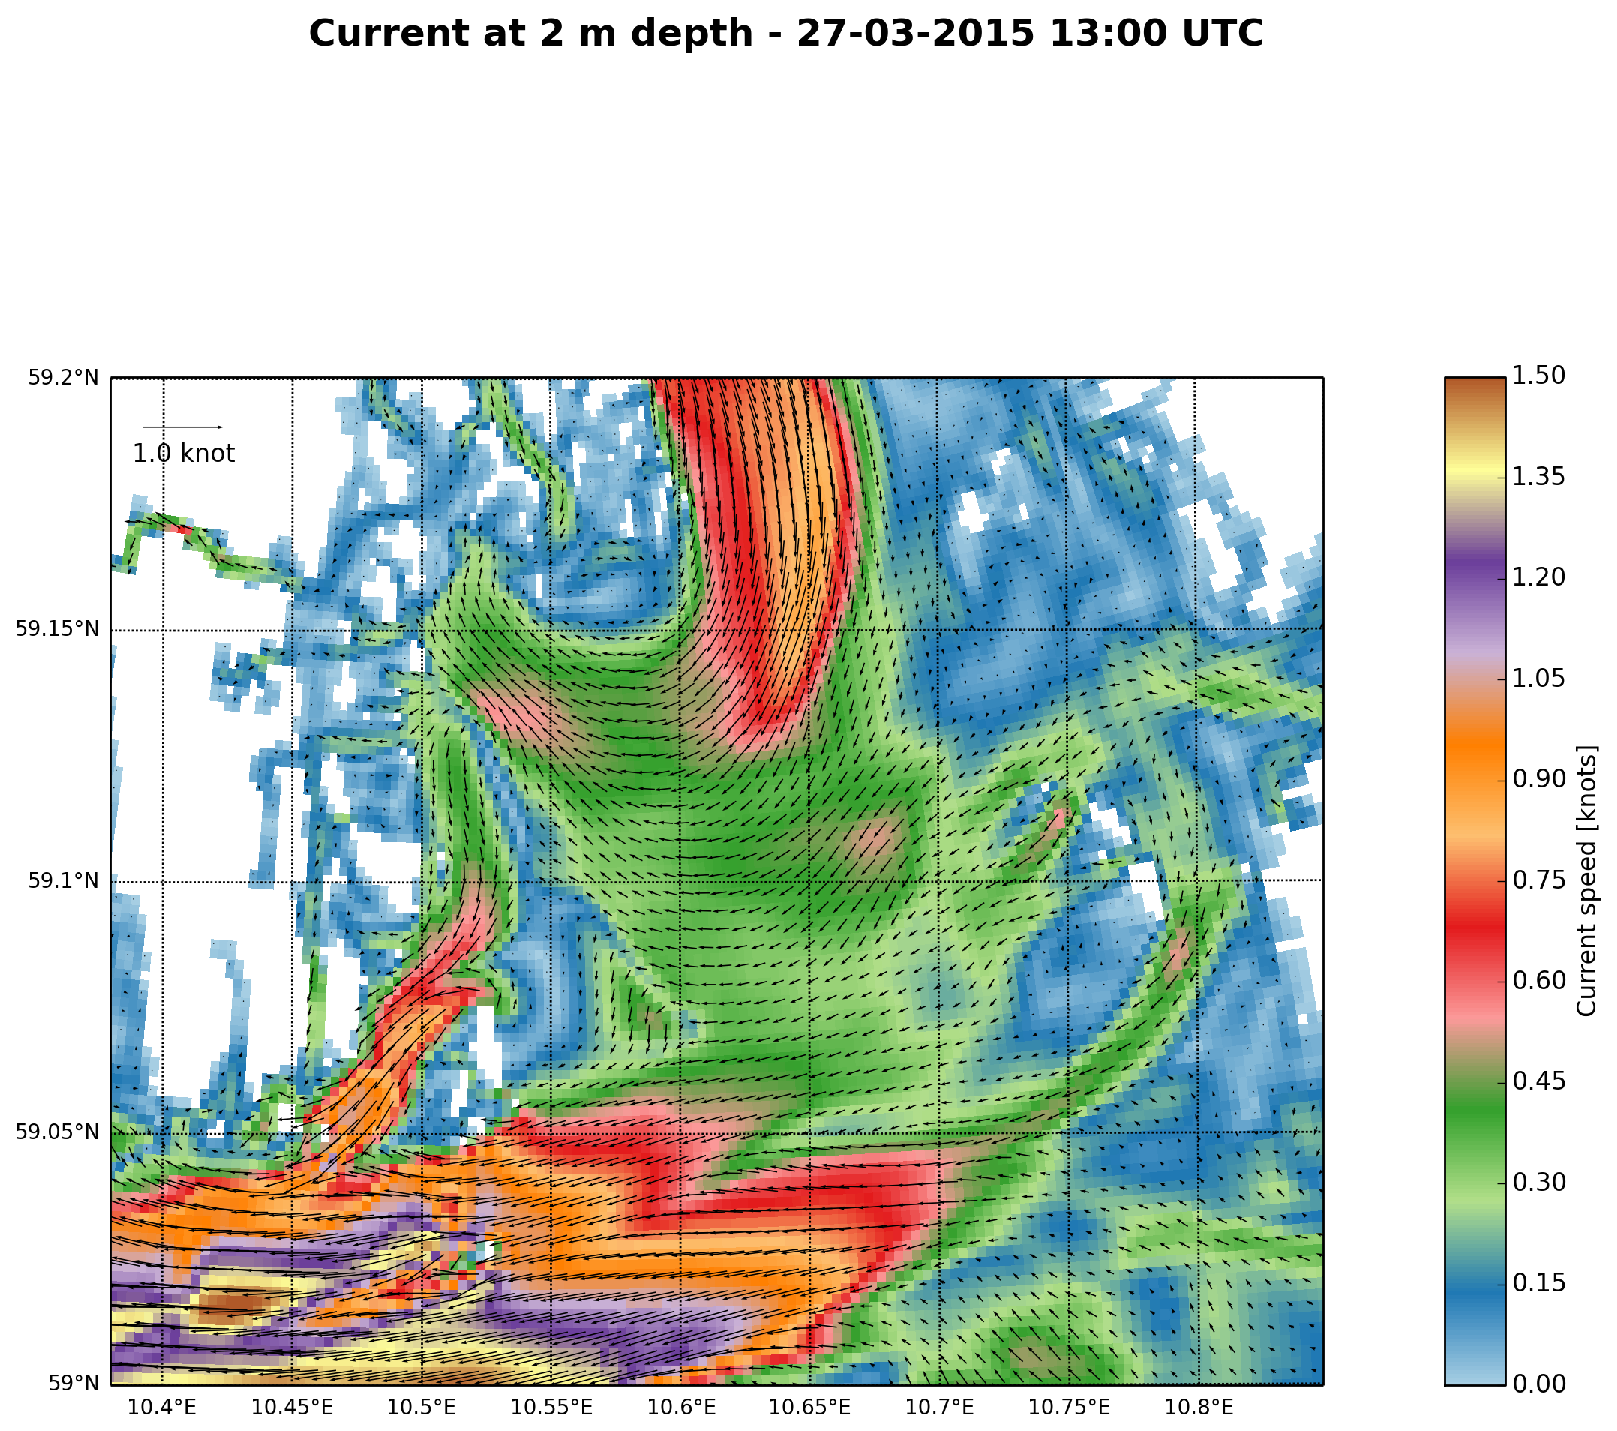
\includegraphics[height=12cm]{kap5/ferder5__0_current_crop}}
  \end{pspicture}
  \caption{\small  As for figure \ref{fig:curr_oslo}, but for the area around the F{\ae}rder lighthouse.  }
  \label{fig:curr_faerder}
\end{figure}

  
 %%%%%%%%%%%%%%%%%%% Figure  %%%%%%%%%%%%%%%
\begin{figure}[t]
  \begin{pspicture}(0,0)(15,16)
% Include graphs
	\rput[b](7.5,0){
\includegraphics[height=16cm]{kap5/drammen1__0_current_crop}}
  \end{pspicture}
  \caption{\small  As for figure \ref{fig:curr_oslo}, but for the Drammensfjord and western Breidangen area.  }
  \label{fig:curr_drammen}
\end{figure}

  

%\subsubsection{Temperature}
 %%%%%%%%%%%%%%%%%%% Figure  %%%%%%%%%%%%%%%
\begin{figure}[t]
  \begin{pspicture}(0,0)(15,12)
% Include graphs
	\rput[b](7.5,0){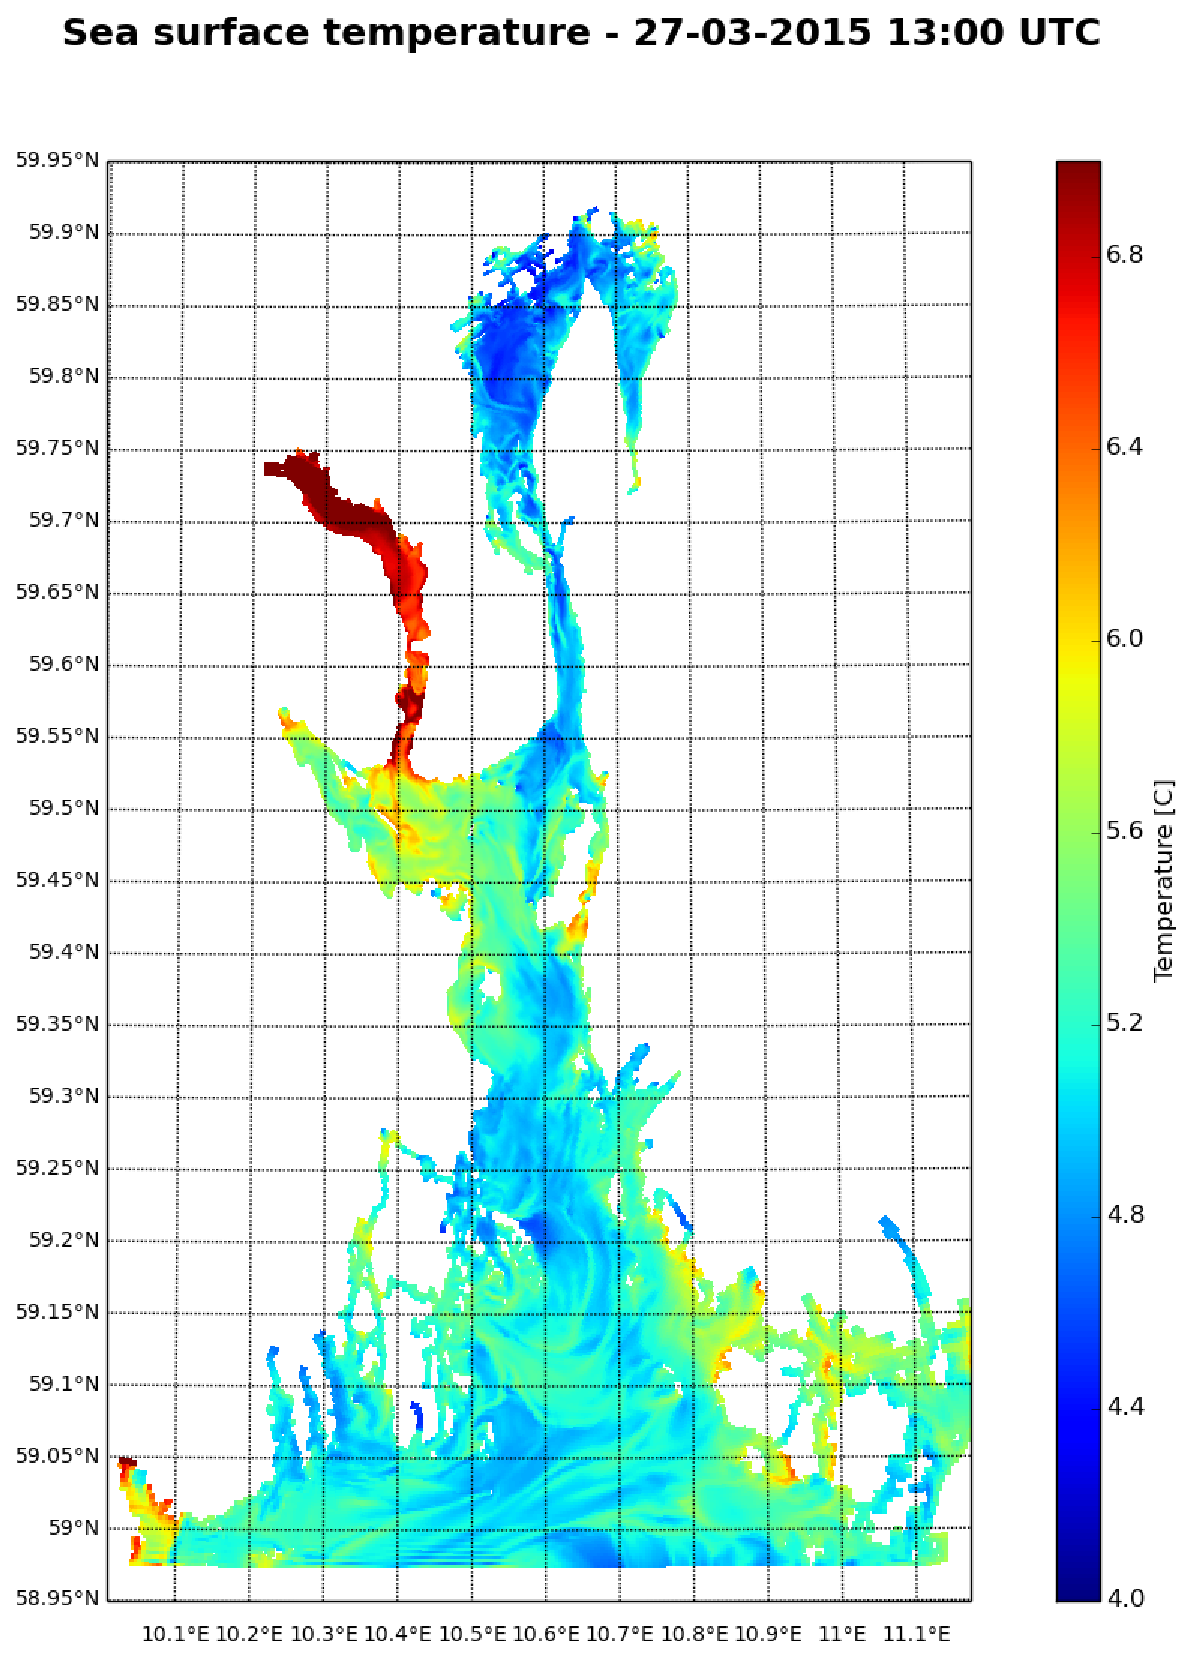
\includegraphics[height=12cm]{kap5/temp_hele_0_current_crop}}
  \end{pspicture}
  \caption{\small  Sea surface temperature (SST) for the entire model domain of the FjordOs model. Note the high SST in the Drammensfjorden area. We believe this is not realistic, and is most likely cause by the mixing up of warmer water from below. This warm water is probably left from imperfect initial conditions. }
  \label{fig:temp_hele}
\end{figure}

  

%\subsubsection{Salinity}
 %%%%%%%%%%%%%%%%%%% Figure  %%%%%%%%%%%%%%%
\begin{figure}[t]
  \begin{pspicture}(0,0)(15,12)
% Include graphs
	\rput[b](7.5,0){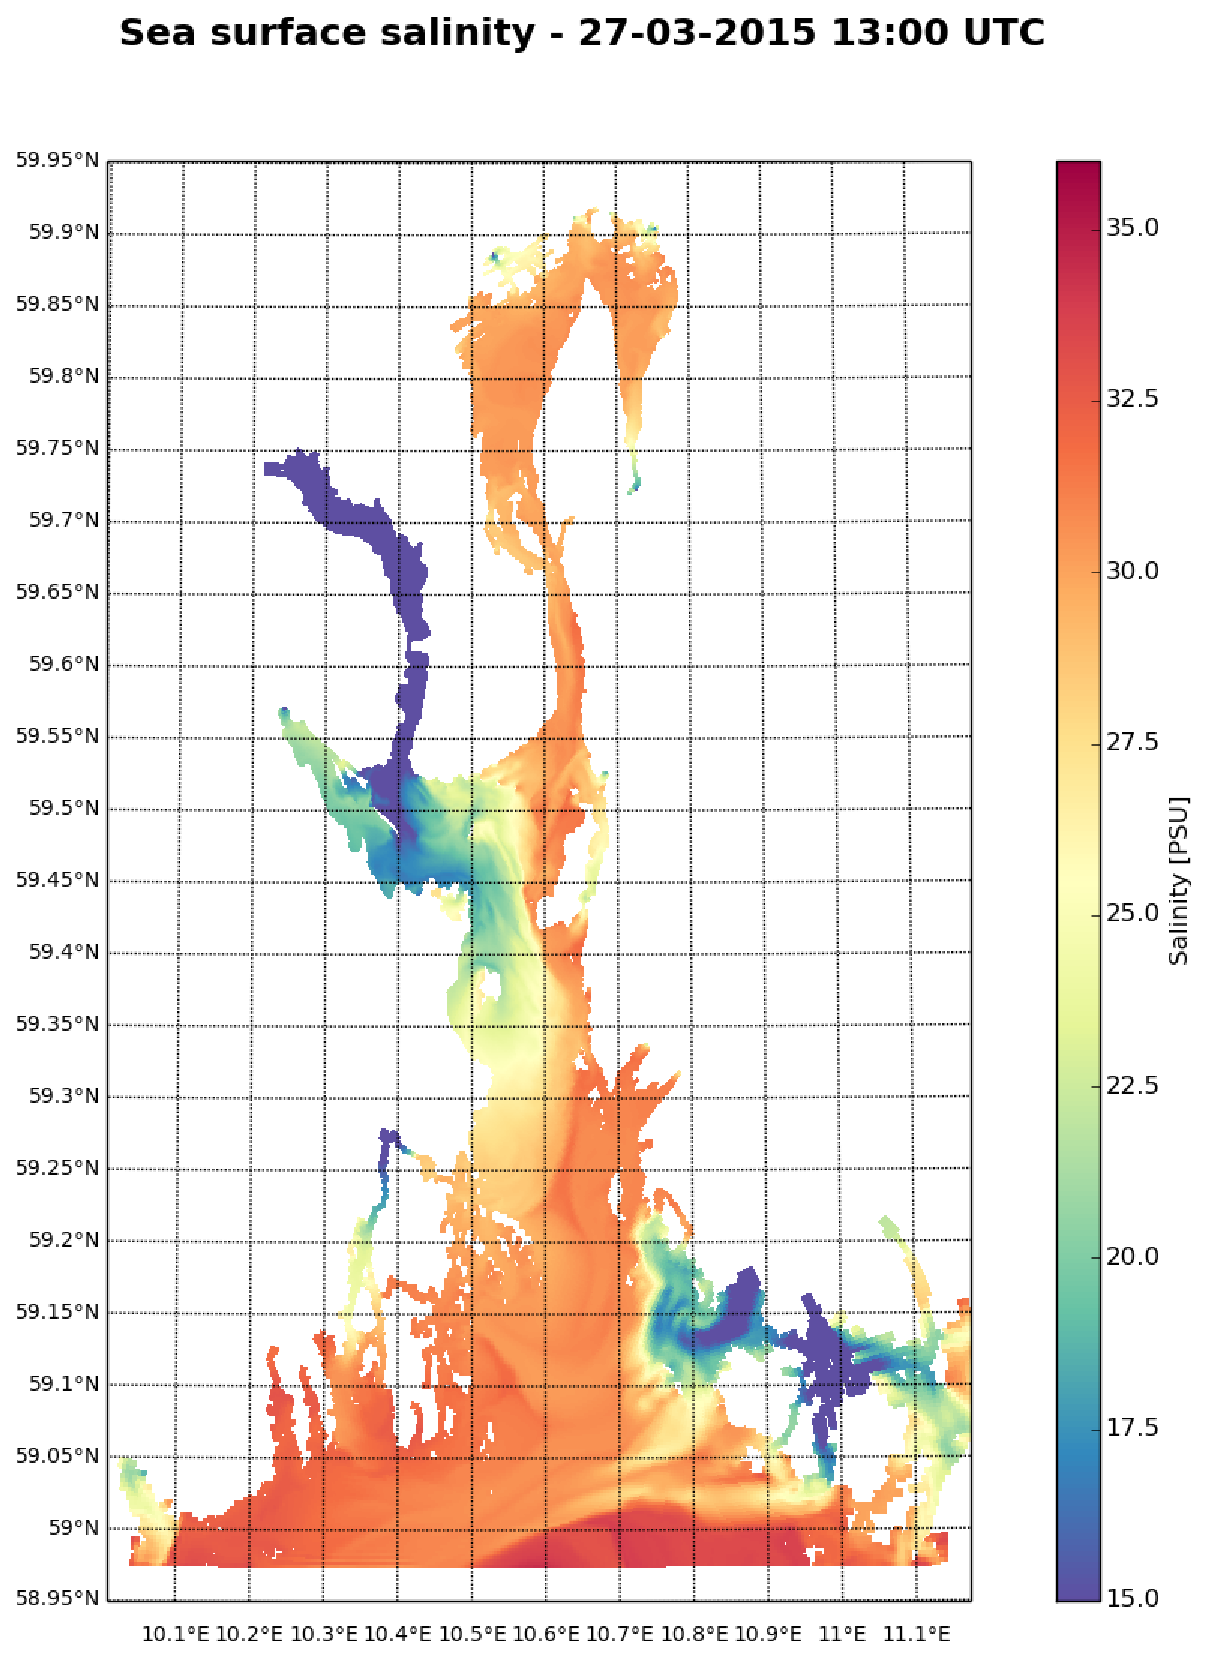
\includegraphics[height=12cm]{kap5/salt_hele_0_current_crop}}
  \end{pspicture}
  \caption{\small  As for figure \ref{fig:temp_hele}, but for sea surface salinity (SSS).  }
  \label{fig:salt_hele}
\end{figure}

  

%\subsubsection{Sea level}
 %%%%%%%%%%%%%%%%%%% Figure  %%%%%%%%%%%%%%%
\begin{figure}[t]
  \begin{pspicture}(0,0)(15,17)
% Include graphs
	\rput[b](7.5,0){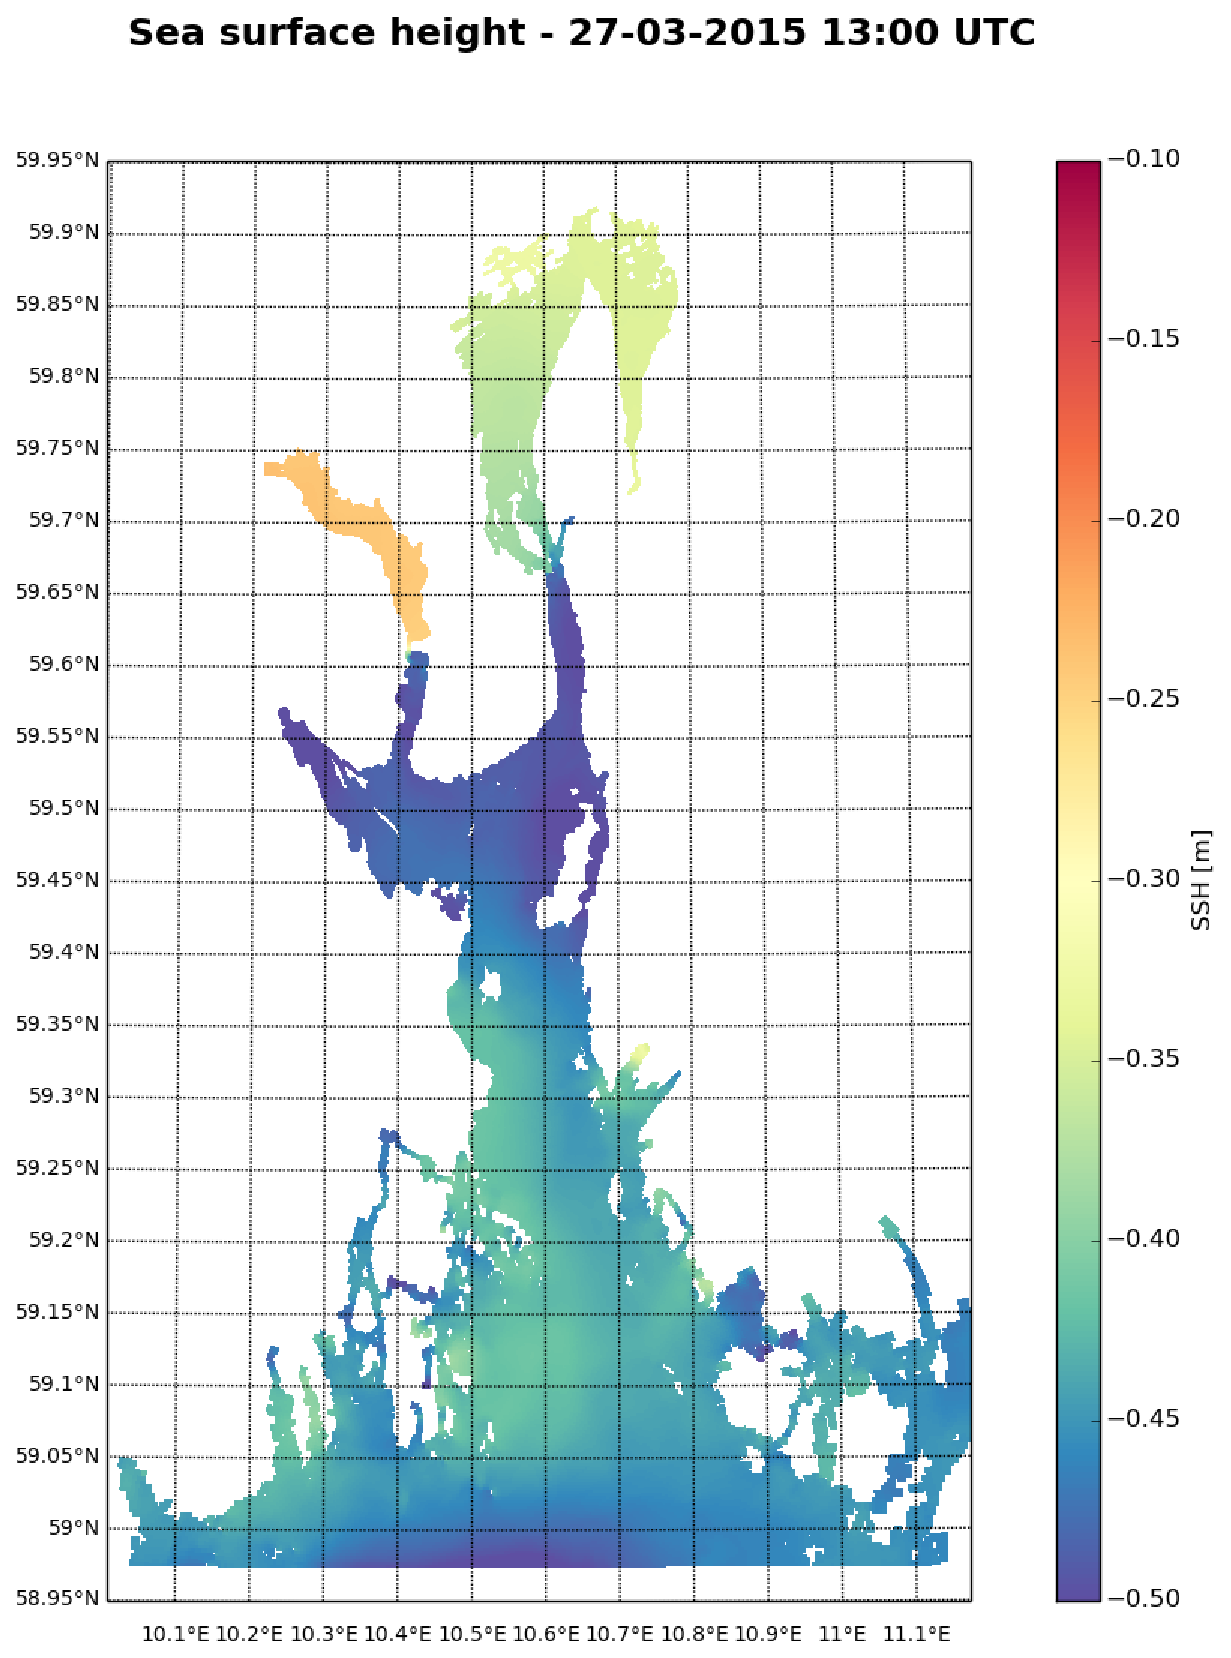
\includegraphics[height=17cm]{kap5/zeta_hele_0_crop}}
  \end{pspicture}
  \caption{\small  As for figure \ref{fig:temp_hele}, but for sea surface height (SSH).  }
  \label{fig:ssh_hele}
\end{figure}

  
